\documentclass[12pt]{article}

\usepackage[utf8]{inputenc}
\usepackage[T1]{fontenc}
\usepackage[catalan]{babel}
\usepackage{lmodern}
\usepackage{geometry}
\usepackage{hyperref}
\usepackage{xcolor}
\usepackage[bf,sf,small,pagestyles]{titlesec}
\usepackage[font={footnotesize, sf}, labelfont=bf]{caption} 
\usepackage{siunitx}
\usepackage{graphicx}
\usepackage{booktabs}
\usepackage{amsmath,amssymb}
\usepackage[catalan]{cleveref}

\geometry{
	a4paper,
	right = 2.5cm,
	left = 2.5cm,
	bottom = 3cm,
	top = 3cm
}

\hypersetup{
	colorlinks,
	linkcolor = {red!50!blue},
	linktoc = page
}

\crefname{figure}{figura}{figures}
\numberwithin{table}{section}
\numberwithin{figure}{section}
\numberwithin{equation}{section}

\graphicspath{{./figs/}}

% Unitats
\sisetup{
	inter-unit-product = \ensuremath{ \cdot },
	allow-number-unit-breaks = true,
	detect-family = true,
	list-final-separator = { i },
	list-units = single
}

\newcommand{\Z}{\mathbb{Z}}
\newcommand{\N}{\mathbb{N}}
\newcommand{\R}{\mathbb{R}}
\newcommand{\abs}[1]{\left\lvert #1 \right\rvert}
\newcommand{\parbreak}{
	\begin{center}
		--- $\ast$ ---
	\end{center} 
}
\makeatletter
\newcommand*{\defeq}{\mathrel{\rlap{%
    \raisebox{0.3ex}{$\m@th\cdot$}}%
  \raisebox{-0.3ex}{$\m@th\cdot$}}%
=}
\makeatother

\newpagestyle{pagina}{
	\headrule
	\sethead*{\sffamily {\bfseries Pràctica 3:} Interpolació polinòmica i integració numèrica}{}{\sffamily \sectiontitle}
	\footrule
	\setfoot*{}{}{\sffamily \thepage}
}
\renewpagestyle{plain}{
	\footrule
	\setfoot*{}{}{\sffamily \thepage}
}
\pagestyle{pagina}

\titleformat{\section}[hang]{\bfseries \sffamily \Large}{}{0pt}{}{\thispagestyle{plain}}

\title{\sffamily {\bfseries Pràctica 3:} Interpolació polinòmica i integració numèrica}
\author{\sffamily Arnau Mas}
\date{\sffamily 24 d'Abril 2018}

\begin{document}
\maketitle

\section{Problema 1}
\begin{figure}[p]
	\centering
	\sffamily \footnotesize
	% GNUPLOT: LaTeX picture with Postscript
\begingroup
  \makeatletter
  \providecommand\color[2][]{%
    \GenericError{(gnuplot) \space\space\space\@spaces}{%
      Package color not loaded in conjunction with
      terminal option `colourtext'%
    }{See the gnuplot documentation for explanation.%
    }{Either use 'blacktext' in gnuplot or load the package
      color.sty in LaTeX.}%
    \renewcommand\color[2][]{}%
  }%
  \providecommand\includegraphics[2][]{%
    \GenericError{(gnuplot) \space\space\space\@spaces}{%
      Package graphicx or graphics not loaded%
    }{See the gnuplot documentation for explanation.%
    }{The gnuplot epslatex terminal needs graphicx.sty or graphics.sty.}%
    \renewcommand\includegraphics[2][]{}%
  }%
  \providecommand\rotatebox[2]{#2}%
  \@ifundefined{ifGPcolor}{%
    \newif\ifGPcolor
    \GPcolortrue
  }{}%
  \@ifundefined{ifGPblacktext}{%
    \newif\ifGPblacktext
    \GPblacktextfalse
  }{}%
  % define a \g@addto@macro without @ in the name:
  \let\gplgaddtomacro\g@addto@macro
  % define empty templates for all commands taking text:
  \gdef\gplbacktext{}%
  \gdef\gplfronttext{}%
  \makeatother
  \ifGPblacktext
    % no textcolor at all
    \def\colorrgb#1{}%
    \def\colorgray#1{}%
  \else
    % gray or color?
    \ifGPcolor
      \def\colorrgb#1{\color[rgb]{#1}}%
      \def\colorgray#1{\color[gray]{#1}}%
      \expandafter\def\csname LTw\endcsname{\color{white}}%
      \expandafter\def\csname LTb\endcsname{\color{black}}%
      \expandafter\def\csname LTa\endcsname{\color{black}}%
      \expandafter\def\csname LT0\endcsname{\color[rgb]{1,0,0}}%
      \expandafter\def\csname LT1\endcsname{\color[rgb]{0,1,0}}%
      \expandafter\def\csname LT2\endcsname{\color[rgb]{0,0,1}}%
      \expandafter\def\csname LT3\endcsname{\color[rgb]{1,0,1}}%
      \expandafter\def\csname LT4\endcsname{\color[rgb]{0,1,1}}%
      \expandafter\def\csname LT5\endcsname{\color[rgb]{1,1,0}}%
      \expandafter\def\csname LT6\endcsname{\color[rgb]{0,0,0}}%
      \expandafter\def\csname LT7\endcsname{\color[rgb]{1,0.3,0}}%
      \expandafter\def\csname LT8\endcsname{\color[rgb]{0.5,0.5,0.5}}%
    \else
      % gray
      \def\colorrgb#1{\color{black}}%
      \def\colorgray#1{\color[gray]{#1}}%
      \expandafter\def\csname LTw\endcsname{\color{white}}%
      \expandafter\def\csname LTb\endcsname{\color{black}}%
      \expandafter\def\csname LTa\endcsname{\color{black}}%
      \expandafter\def\csname LT0\endcsname{\color{black}}%
      \expandafter\def\csname LT1\endcsname{\color{black}}%
      \expandafter\def\csname LT2\endcsname{\color{black}}%
      \expandafter\def\csname LT3\endcsname{\color{black}}%
      \expandafter\def\csname LT4\endcsname{\color{black}}%
      \expandafter\def\csname LT5\endcsname{\color{black}}%
      \expandafter\def\csname LT6\endcsname{\color{black}}%
      \expandafter\def\csname LT7\endcsname{\color{black}}%
      \expandafter\def\csname LT8\endcsname{\color{black}}%
    \fi
  \fi
    \setlength{\unitlength}{0.0500bp}%
    \ifx\gptboxheight\undefined%
      \newlength{\gptboxheight}%
      \newlength{\gptboxwidth}%
      \newsavebox{\gptboxtext}%
    \fi%
    \setlength{\fboxrule}{0.5pt}%
    \setlength{\fboxsep}{1pt}%
\begin{picture}(4534.00,2834.00)%
    \gplgaddtomacro\gplbacktext{%
      \csname LTb\endcsname%%
      \put(990,499){\makebox(0,0)[r]{\strut{}\num{-0.25}}}%
      \put(990,842){\makebox(0,0)[r]{\strut{}\num{0}}}%
      \put(990,1184){\makebox(0,0)[r]{\strut{}\num{0.25}}}%
      \put(990,1527){\makebox(0,0)[r]{\strut{}\num{0.5}}}%
      \put(990,1869){\makebox(0,0)[r]{\strut{}\num{0.75}}}%
      \put(990,2212){\makebox(0,0)[r]{\strut{}\num{1}}}%
      \put(990,2554){\makebox(0,0)[r]{\strut{}\num{1.25}}}%
      \put(1259,279){\makebox(0,0){\strut{}\num{-1}}}%
      \put(1944,279){\makebox(0,0){\strut{}\num{-0.5}}}%
      \put(2630,279){\makebox(0,0){\strut{}\num{0}}}%
      \put(3315,279){\makebox(0,0){\strut{}\num{0.5}}}%
      \put(4000,279){\makebox(0,0){\strut{}\num{1}}}%
      \put(2355,855){\makebox(0,0)[l]{\strut{}$ n = 4 $}}%
    }%
    \gplgaddtomacro\gplfronttext{%
    }%
    \gplbacktext
    \put(0,0){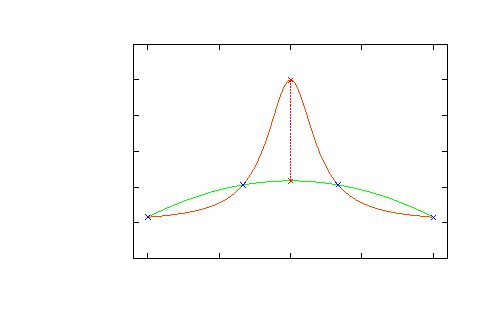
\includegraphics{04-eq}}%
    \gplfronttext
  \end{picture}%
\endgroup
% GNUPLOT: LaTeX picture with Postscript
\begingroup
  \makeatletter
  \providecommand\color[2][]{%
    \GenericError{(gnuplot) \space\space\space\@spaces}{%
      Package color not loaded in conjunction with
      terminal option `colourtext'%
    }{See the gnuplot documentation for explanation.%
    }{Either use 'blacktext' in gnuplot or load the package
      color.sty in LaTeX.}%
    \renewcommand\color[2][]{}%
  }%
  \providecommand\includegraphics[2][]{%
    \GenericError{(gnuplot) \space\space\space\@spaces}{%
      Package graphicx or graphics not loaded%
    }{See the gnuplot documentation for explanation.%
    }{The gnuplot epslatex terminal needs graphicx.sty or graphics.sty.}%
    \renewcommand\includegraphics[2][]{}%
  }%
  \providecommand\rotatebox[2]{#2}%
  \@ifundefined{ifGPcolor}{%
    \newif\ifGPcolor
    \GPcolortrue
  }{}%
  \@ifundefined{ifGPblacktext}{%
    \newif\ifGPblacktext
    \GPblacktextfalse
  }{}%
  % define a \g@addto@macro without @ in the name:
  \let\gplgaddtomacro\g@addto@macro
  % define empty templates for all commands taking text:
  \gdef\gplbacktext{}%
  \gdef\gplfronttext{}%
  \makeatother
  \ifGPblacktext
    % no textcolor at all
    \def\colorrgb#1{}%
    \def\colorgray#1{}%
  \else
    % gray or color?
    \ifGPcolor
      \def\colorrgb#1{\color[rgb]{#1}}%
      \def\colorgray#1{\color[gray]{#1}}%
      \expandafter\def\csname LTw\endcsname{\color{white}}%
      \expandafter\def\csname LTb\endcsname{\color{black}}%
      \expandafter\def\csname LTa\endcsname{\color{black}}%
      \expandafter\def\csname LT0\endcsname{\color[rgb]{1,0,0}}%
      \expandafter\def\csname LT1\endcsname{\color[rgb]{0,1,0}}%
      \expandafter\def\csname LT2\endcsname{\color[rgb]{0,0,1}}%
      \expandafter\def\csname LT3\endcsname{\color[rgb]{1,0,1}}%
      \expandafter\def\csname LT4\endcsname{\color[rgb]{0,1,1}}%
      \expandafter\def\csname LT5\endcsname{\color[rgb]{1,1,0}}%
      \expandafter\def\csname LT6\endcsname{\color[rgb]{0,0,0}}%
      \expandafter\def\csname LT7\endcsname{\color[rgb]{1,0.3,0}}%
      \expandafter\def\csname LT8\endcsname{\color[rgb]{0.5,0.5,0.5}}%
    \else
      % gray
      \def\colorrgb#1{\color{black}}%
      \def\colorgray#1{\color[gray]{#1}}%
      \expandafter\def\csname LTw\endcsname{\color{white}}%
      \expandafter\def\csname LTb\endcsname{\color{black}}%
      \expandafter\def\csname LTa\endcsname{\color{black}}%
      \expandafter\def\csname LT0\endcsname{\color{black}}%
      \expandafter\def\csname LT1\endcsname{\color{black}}%
      \expandafter\def\csname LT2\endcsname{\color{black}}%
      \expandafter\def\csname LT3\endcsname{\color{black}}%
      \expandafter\def\csname LT4\endcsname{\color{black}}%
      \expandafter\def\csname LT5\endcsname{\color{black}}%
      \expandafter\def\csname LT6\endcsname{\color{black}}%
      \expandafter\def\csname LT7\endcsname{\color{black}}%
      \expandafter\def\csname LT8\endcsname{\color{black}}%
    \fi
  \fi
    \setlength{\unitlength}{0.0500bp}%
    \ifx\gptboxheight\undefined%
      \newlength{\gptboxheight}%
      \newlength{\gptboxwidth}%
      \newsavebox{\gptboxtext}%
    \fi%
    \setlength{\fboxrule}{0.5pt}%
    \setlength{\fboxsep}{1pt}%
\begin{picture}(4534.00,2834.00)%
    \gplgaddtomacro\gplbacktext{%
      \csname LTb\endcsname%%
      \put(990,499){\makebox(0,0)[r]{\strut{}\num{-0.25}}}%
      \put(990,842){\makebox(0,0)[r]{\strut{}\num{0}}}%
      \put(990,1184){\makebox(0,0)[r]{\strut{}\num{0.25}}}%
      \put(990,1527){\makebox(0,0)[r]{\strut{}\num{0.5}}}%
      \put(990,1869){\makebox(0,0)[r]{\strut{}\num{0.75}}}%
      \put(990,2212){\makebox(0,0)[r]{\strut{}\num{1}}}%
      \put(990,2554){\makebox(0,0)[r]{\strut{}\num{1.25}}}%
      \put(1259,279){\makebox(0,0){\strut{}\num{-1}}}%
      \put(1944,279){\makebox(0,0){\strut{}\num{-0.5}}}%
      \put(2630,279){\makebox(0,0){\strut{}\num{0}}}%
      \put(3315,279){\makebox(0,0){\strut{}\num{0.5}}}%
      \put(4000,279){\makebox(0,0){\strut{}\num{1}}}%
      \put(2355,855){\makebox(0,0)[l]{\strut{}$ n = 4 $}}%
    }%
    \gplgaddtomacro\gplfronttext{%
    }%
    \gplbacktext
    \put(0,0){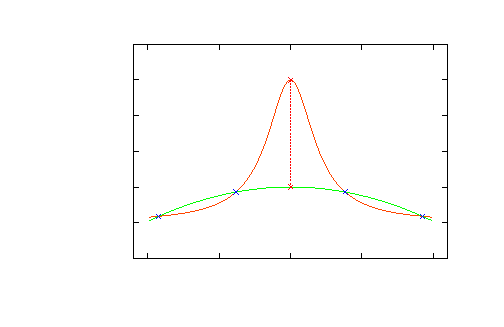
\includegraphics{04-cheb}}%
    \gplfronttext
  \end{picture}%
\endgroup

	% GNUPLOT: LaTeX picture with Postscript
\begingroup
  \makeatletter
  \providecommand\color[2][]{%
    \GenericError{(gnuplot) \space\space\space\@spaces}{%
      Package color not loaded in conjunction with
      terminal option `colourtext'%
    }{See the gnuplot documentation for explanation.%
    }{Either use 'blacktext' in gnuplot or load the package
      color.sty in LaTeX.}%
    \renewcommand\color[2][]{}%
  }%
  \providecommand\includegraphics[2][]{%
    \GenericError{(gnuplot) \space\space\space\@spaces}{%
      Package graphicx or graphics not loaded%
    }{See the gnuplot documentation for explanation.%
    }{The gnuplot epslatex terminal needs graphicx.sty or graphics.sty.}%
    \renewcommand\includegraphics[2][]{}%
  }%
  \providecommand\rotatebox[2]{#2}%
  \@ifundefined{ifGPcolor}{%
    \newif\ifGPcolor
    \GPcolortrue
  }{}%
  \@ifundefined{ifGPblacktext}{%
    \newif\ifGPblacktext
    \GPblacktextfalse
  }{}%
  % define a \g@addto@macro without @ in the name:
  \let\gplgaddtomacro\g@addto@macro
  % define empty templates for all commands taking text:
  \gdef\gplbacktext{}%
  \gdef\gplfronttext{}%
  \makeatother
  \ifGPblacktext
    % no textcolor at all
    \def\colorrgb#1{}%
    \def\colorgray#1{}%
  \else
    % gray or color?
    \ifGPcolor
      \def\colorrgb#1{\color[rgb]{#1}}%
      \def\colorgray#1{\color[gray]{#1}}%
      \expandafter\def\csname LTw\endcsname{\color{white}}%
      \expandafter\def\csname LTb\endcsname{\color{black}}%
      \expandafter\def\csname LTa\endcsname{\color{black}}%
      \expandafter\def\csname LT0\endcsname{\color[rgb]{1,0,0}}%
      \expandafter\def\csname LT1\endcsname{\color[rgb]{0,1,0}}%
      \expandafter\def\csname LT2\endcsname{\color[rgb]{0,0,1}}%
      \expandafter\def\csname LT3\endcsname{\color[rgb]{1,0,1}}%
      \expandafter\def\csname LT4\endcsname{\color[rgb]{0,1,1}}%
      \expandafter\def\csname LT5\endcsname{\color[rgb]{1,1,0}}%
      \expandafter\def\csname LT6\endcsname{\color[rgb]{0,0,0}}%
      \expandafter\def\csname LT7\endcsname{\color[rgb]{1,0.3,0}}%
      \expandafter\def\csname LT8\endcsname{\color[rgb]{0.5,0.5,0.5}}%
    \else
      % gray
      \def\colorrgb#1{\color{black}}%
      \def\colorgray#1{\color[gray]{#1}}%
      \expandafter\def\csname LTw\endcsname{\color{white}}%
      \expandafter\def\csname LTb\endcsname{\color{black}}%
      \expandafter\def\csname LTa\endcsname{\color{black}}%
      \expandafter\def\csname LT0\endcsname{\color{black}}%
      \expandafter\def\csname LT1\endcsname{\color{black}}%
      \expandafter\def\csname LT2\endcsname{\color{black}}%
      \expandafter\def\csname LT3\endcsname{\color{black}}%
      \expandafter\def\csname LT4\endcsname{\color{black}}%
      \expandafter\def\csname LT5\endcsname{\color{black}}%
      \expandafter\def\csname LT6\endcsname{\color{black}}%
      \expandafter\def\csname LT7\endcsname{\color{black}}%
      \expandafter\def\csname LT8\endcsname{\color{black}}%
    \fi
  \fi
    \setlength{\unitlength}{0.0500bp}%
    \ifx\gptboxheight\undefined%
      \newlength{\gptboxheight}%
      \newlength{\gptboxwidth}%
      \newsavebox{\gptboxtext}%
    \fi%
    \setlength{\fboxrule}{0.5pt}%
    \setlength{\fboxsep}{1pt}%
\begin{picture}(3968.00,3968.00)%
    \gplgaddtomacro\gplbacktext{%
      \csname LTb\endcsname%%
      \put(726,440){\makebox(0,0)[r]{\strut{}\num{0}}}%
      \put(726,991){\makebox(0,0)[r]{\strut{}\num{0.2}}}%
      \put(726,1542){\makebox(0,0)[r]{\strut{}\num{0.4}}}%
      \put(726,2094){\makebox(0,0)[r]{\strut{}\num{0.6}}}%
      \put(726,2645){\makebox(0,0)[r]{\strut{}\num{0.8}}}%
      \put(726,3196){\makebox(0,0)[r]{\strut{}\num{1}}}%
      \put(726,3747){\makebox(0,0)[r]{\strut{}\num{1.2}}}%
      \put(981,220){\makebox(0,0){\strut{}\num{-1}}}%
      \put(1598,220){\makebox(0,0){\strut{}\num{-0.5}}}%
      \put(2215,220){\makebox(0,0){\strut{}\num{0}}}%
      \put(2831,220){\makebox(0,0){\strut{}\num{0.5}}}%
      \put(3448,220){\makebox(0,0){\strut{}\num{1}}}%
    }%
    \gplgaddtomacro\gplfronttext{%
    }%
    \gplbacktext
    \put(0,0){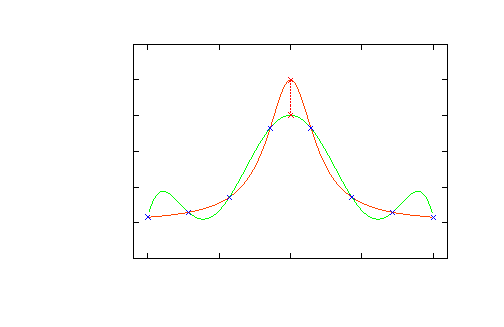
\includegraphics{08-eq}}%
    \gplfronttext
  \end{picture}%
\endgroup
% GNUPLOT: LaTeX picture with Postscript
\begingroup
  \makeatletter
  \providecommand\color[2][]{%
    \GenericError{(gnuplot) \space\space\space\@spaces}{%
      Package color not loaded in conjunction with
      terminal option `colourtext'%
    }{See the gnuplot documentation for explanation.%
    }{Either use 'blacktext' in gnuplot or load the package
      color.sty in LaTeX.}%
    \renewcommand\color[2][]{}%
  }%
  \providecommand\includegraphics[2][]{%
    \GenericError{(gnuplot) \space\space\space\@spaces}{%
      Package graphicx or graphics not loaded%
    }{See the gnuplot documentation for explanation.%
    }{The gnuplot epslatex terminal needs graphicx.sty or graphics.sty.}%
    \renewcommand\includegraphics[2][]{}%
  }%
  \providecommand\rotatebox[2]{#2}%
  \@ifundefined{ifGPcolor}{%
    \newif\ifGPcolor
    \GPcolortrue
  }{}%
  \@ifundefined{ifGPblacktext}{%
    \newif\ifGPblacktext
    \GPblacktextfalse
  }{}%
  % define a \g@addto@macro without @ in the name:
  \let\gplgaddtomacro\g@addto@macro
  % define empty templates for all commands taking text:
  \gdef\gplbacktext{}%
  \gdef\gplfronttext{}%
  \makeatother
  \ifGPblacktext
    % no textcolor at all
    \def\colorrgb#1{}%
    \def\colorgray#1{}%
  \else
    % gray or color?
    \ifGPcolor
      \def\colorrgb#1{\color[rgb]{#1}}%
      \def\colorgray#1{\color[gray]{#1}}%
      \expandafter\def\csname LTw\endcsname{\color{white}}%
      \expandafter\def\csname LTb\endcsname{\color{black}}%
      \expandafter\def\csname LTa\endcsname{\color{black}}%
      \expandafter\def\csname LT0\endcsname{\color[rgb]{1,0,0}}%
      \expandafter\def\csname LT1\endcsname{\color[rgb]{0,1,0}}%
      \expandafter\def\csname LT2\endcsname{\color[rgb]{0,0,1}}%
      \expandafter\def\csname LT3\endcsname{\color[rgb]{1,0,1}}%
      \expandafter\def\csname LT4\endcsname{\color[rgb]{0,1,1}}%
      \expandafter\def\csname LT5\endcsname{\color[rgb]{1,1,0}}%
      \expandafter\def\csname LT6\endcsname{\color[rgb]{0,0,0}}%
      \expandafter\def\csname LT7\endcsname{\color[rgb]{1,0.3,0}}%
      \expandafter\def\csname LT8\endcsname{\color[rgb]{0.5,0.5,0.5}}%
    \else
      % gray
      \def\colorrgb#1{\color{black}}%
      \def\colorgray#1{\color[gray]{#1}}%
      \expandafter\def\csname LTw\endcsname{\color{white}}%
      \expandafter\def\csname LTb\endcsname{\color{black}}%
      \expandafter\def\csname LTa\endcsname{\color{black}}%
      \expandafter\def\csname LT0\endcsname{\color{black}}%
      \expandafter\def\csname LT1\endcsname{\color{black}}%
      \expandafter\def\csname LT2\endcsname{\color{black}}%
      \expandafter\def\csname LT3\endcsname{\color{black}}%
      \expandafter\def\csname LT4\endcsname{\color{black}}%
      \expandafter\def\csname LT5\endcsname{\color{black}}%
      \expandafter\def\csname LT6\endcsname{\color{black}}%
      \expandafter\def\csname LT7\endcsname{\color{black}}%
      \expandafter\def\csname LT8\endcsname{\color{black}}%
    \fi
  \fi
    \setlength{\unitlength}{0.0500bp}%
    \ifx\gptboxheight\undefined%
      \newlength{\gptboxheight}%
      \newlength{\gptboxwidth}%
      \newsavebox{\gptboxtext}%
    \fi%
    \setlength{\fboxrule}{0.5pt}%
    \setlength{\fboxsep}{1pt}%
\begin{picture}(3968.00,3968.00)%
    \gplgaddtomacro\gplbacktext{%
      \csname LTb\endcsname%%
      \put(726,440){\makebox(0,0)[r]{\strut{}\num{0}}}%
      \put(726,991){\makebox(0,0)[r]{\strut{}\num{0.2}}}%
      \put(726,1542){\makebox(0,0)[r]{\strut{}\num{0.4}}}%
      \put(726,2094){\makebox(0,0)[r]{\strut{}\num{0.6}}}%
      \put(726,2645){\makebox(0,0)[r]{\strut{}\num{0.8}}}%
      \put(726,3196){\makebox(0,0)[r]{\strut{}\num{1}}}%
      \put(726,3747){\makebox(0,0)[r]{\strut{}\num{1.2}}}%
      \put(981,220){\makebox(0,0){\strut{}\num{-1}}}%
      \put(1598,220){\makebox(0,0){\strut{}\num{-0.5}}}%
      \put(2215,220){\makebox(0,0){\strut{}\num{0}}}%
      \put(2831,220){\makebox(0,0){\strut{}\num{0.5}}}%
      \put(3448,220){\makebox(0,0){\strut{}\num{1}}}%
    }%
    \gplgaddtomacro\gplfronttext{%
    }%
    \gplbacktext
    \put(0,0){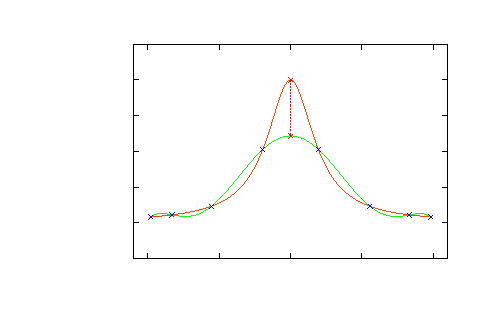
\includegraphics{08-cheb}}%
    \gplfronttext
  \end{picture}%
\endgroup

	% GNUPLOT: LaTeX picture with Postscript
\begingroup
  \makeatletter
  \providecommand\color[2][]{%
    \GenericError{(gnuplot) \space\space\space\@spaces}{%
      Package color not loaded in conjunction with
      terminal option `colourtext'%
    }{See the gnuplot documentation for explanation.%
    }{Either use 'blacktext' in gnuplot or load the package
      color.sty in LaTeX.}%
    \renewcommand\color[2][]{}%
  }%
  \providecommand\includegraphics[2][]{%
    \GenericError{(gnuplot) \space\space\space\@spaces}{%
      Package graphicx or graphics not loaded%
    }{See the gnuplot documentation for explanation.%
    }{The gnuplot epslatex terminal needs graphicx.sty or graphics.sty.}%
    \renewcommand\includegraphics[2][]{}%
  }%
  \providecommand\rotatebox[2]{#2}%
  \@ifundefined{ifGPcolor}{%
    \newif\ifGPcolor
    \GPcolortrue
  }{}%
  \@ifundefined{ifGPblacktext}{%
    \newif\ifGPblacktext
    \GPblacktextfalse
  }{}%
  % define a \g@addto@macro without @ in the name:
  \let\gplgaddtomacro\g@addto@macro
  % define empty templates for all commands taking text:
  \gdef\gplbacktext{}%
  \gdef\gplfronttext{}%
  \makeatother
  \ifGPblacktext
    % no textcolor at all
    \def\colorrgb#1{}%
    \def\colorgray#1{}%
  \else
    % gray or color?
    \ifGPcolor
      \def\colorrgb#1{\color[rgb]{#1}}%
      \def\colorgray#1{\color[gray]{#1}}%
      \expandafter\def\csname LTw\endcsname{\color{white}}%
      \expandafter\def\csname LTb\endcsname{\color{black}}%
      \expandafter\def\csname LTa\endcsname{\color{black}}%
      \expandafter\def\csname LT0\endcsname{\color[rgb]{1,0,0}}%
      \expandafter\def\csname LT1\endcsname{\color[rgb]{0,1,0}}%
      \expandafter\def\csname LT2\endcsname{\color[rgb]{0,0,1}}%
      \expandafter\def\csname LT3\endcsname{\color[rgb]{1,0,1}}%
      \expandafter\def\csname LT4\endcsname{\color[rgb]{0,1,1}}%
      \expandafter\def\csname LT5\endcsname{\color[rgb]{1,1,0}}%
      \expandafter\def\csname LT6\endcsname{\color[rgb]{0,0,0}}%
      \expandafter\def\csname LT7\endcsname{\color[rgb]{1,0.3,0}}%
      \expandafter\def\csname LT8\endcsname{\color[rgb]{0.5,0.5,0.5}}%
    \else
      % gray
      \def\colorrgb#1{\color{black}}%
      \def\colorgray#1{\color[gray]{#1}}%
      \expandafter\def\csname LTw\endcsname{\color{white}}%
      \expandafter\def\csname LTb\endcsname{\color{black}}%
      \expandafter\def\csname LTa\endcsname{\color{black}}%
      \expandafter\def\csname LT0\endcsname{\color{black}}%
      \expandafter\def\csname LT1\endcsname{\color{black}}%
      \expandafter\def\csname LT2\endcsname{\color{black}}%
      \expandafter\def\csname LT3\endcsname{\color{black}}%
      \expandafter\def\csname LT4\endcsname{\color{black}}%
      \expandafter\def\csname LT5\endcsname{\color{black}}%
      \expandafter\def\csname LT6\endcsname{\color{black}}%
      \expandafter\def\csname LT7\endcsname{\color{black}}%
      \expandafter\def\csname LT8\endcsname{\color{black}}%
    \fi
  \fi
    \setlength{\unitlength}{0.0500bp}%
    \ifx\gptboxheight\undefined%
      \newlength{\gptboxheight}%
      \newlength{\gptboxwidth}%
      \newsavebox{\gptboxtext}%
    \fi%
    \setlength{\fboxrule}{0.5pt}%
    \setlength{\fboxsep}{1pt}%
\begin{picture}(4534.00,2834.00)%
    \gplgaddtomacro\gplbacktext{%
      \csname LTb\endcsname%%
      \put(990,499){\makebox(0,0)[r]{\strut{}\num{-0.25}}}%
      \put(990,842){\makebox(0,0)[r]{\strut{}\num{0}}}%
      \put(990,1184){\makebox(0,0)[r]{\strut{}\num{0.25}}}%
      \put(990,1527){\makebox(0,0)[r]{\strut{}\num{0.5}}}%
      \put(990,1869){\makebox(0,0)[r]{\strut{}\num{0.75}}}%
      \put(990,2212){\makebox(0,0)[r]{\strut{}\num{1}}}%
      \put(990,2554){\makebox(0,0)[r]{\strut{}\num{1.25}}}%
      \put(1259,279){\makebox(0,0){\strut{}\num{-1}}}%
      \put(1944,279){\makebox(0,0){\strut{}\num{-0.5}}}%
      \put(2630,279){\makebox(0,0){\strut{}\num{0}}}%
      \put(3315,279){\makebox(0,0){\strut{}\num{0.5}}}%
      \put(4000,279){\makebox(0,0){\strut{}\num{1}}}%
      \put(2355,855){\makebox(0,0)[l]{\strut{}$ n = 16 $}}%
      \put(2355,855){\makebox(0,0)[l]{\strut{}$ n = 16 $}}%
    }%
    \gplgaddtomacro\gplfronttext{%
    }%
    \gplbacktext
    \put(0,0){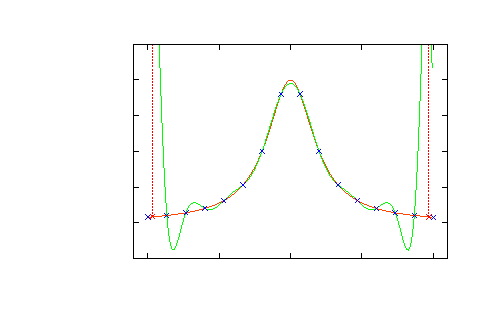
\includegraphics{16-eq}}%
    \gplfronttext
  \end{picture}%
\endgroup
% GNUPLOT: LaTeX picture with Postscript
\begingroup
  \makeatletter
  \providecommand\color[2][]{%
    \GenericError{(gnuplot) \space\space\space\@spaces}{%
      Package color not loaded in conjunction with
      terminal option `colourtext'%
    }{See the gnuplot documentation for explanation.%
    }{Either use 'blacktext' in gnuplot or load the package
      color.sty in LaTeX.}%
    \renewcommand\color[2][]{}%
  }%
  \providecommand\includegraphics[2][]{%
    \GenericError{(gnuplot) \space\space\space\@spaces}{%
      Package graphicx or graphics not loaded%
    }{See the gnuplot documentation for explanation.%
    }{The gnuplot epslatex terminal needs graphicx.sty or graphics.sty.}%
    \renewcommand\includegraphics[2][]{}%
  }%
  \providecommand\rotatebox[2]{#2}%
  \@ifundefined{ifGPcolor}{%
    \newif\ifGPcolor
    \GPcolortrue
  }{}%
  \@ifundefined{ifGPblacktext}{%
    \newif\ifGPblacktext
    \GPblacktextfalse
  }{}%
  % define a \g@addto@macro without @ in the name:
  \let\gplgaddtomacro\g@addto@macro
  % define empty templates for all commands taking text:
  \gdef\gplbacktext{}%
  \gdef\gplfronttext{}%
  \makeatother
  \ifGPblacktext
    % no textcolor at all
    \def\colorrgb#1{}%
    \def\colorgray#1{}%
  \else
    % gray or color?
    \ifGPcolor
      \def\colorrgb#1{\color[rgb]{#1}}%
      \def\colorgray#1{\color[gray]{#1}}%
      \expandafter\def\csname LTw\endcsname{\color{white}}%
      \expandafter\def\csname LTb\endcsname{\color{black}}%
      \expandafter\def\csname LTa\endcsname{\color{black}}%
      \expandafter\def\csname LT0\endcsname{\color[rgb]{1,0,0}}%
      \expandafter\def\csname LT1\endcsname{\color[rgb]{0,1,0}}%
      \expandafter\def\csname LT2\endcsname{\color[rgb]{0,0,1}}%
      \expandafter\def\csname LT3\endcsname{\color[rgb]{1,0,1}}%
      \expandafter\def\csname LT4\endcsname{\color[rgb]{0,1,1}}%
      \expandafter\def\csname LT5\endcsname{\color[rgb]{1,1,0}}%
      \expandafter\def\csname LT6\endcsname{\color[rgb]{0,0,0}}%
      \expandafter\def\csname LT7\endcsname{\color[rgb]{1,0.3,0}}%
      \expandafter\def\csname LT8\endcsname{\color[rgb]{0.5,0.5,0.5}}%
    \else
      % gray
      \def\colorrgb#1{\color{black}}%
      \def\colorgray#1{\color[gray]{#1}}%
      \expandafter\def\csname LTw\endcsname{\color{white}}%
      \expandafter\def\csname LTb\endcsname{\color{black}}%
      \expandafter\def\csname LTa\endcsname{\color{black}}%
      \expandafter\def\csname LT0\endcsname{\color{black}}%
      \expandafter\def\csname LT1\endcsname{\color{black}}%
      \expandafter\def\csname LT2\endcsname{\color{black}}%
      \expandafter\def\csname LT3\endcsname{\color{black}}%
      \expandafter\def\csname LT4\endcsname{\color{black}}%
      \expandafter\def\csname LT5\endcsname{\color{black}}%
      \expandafter\def\csname LT6\endcsname{\color{black}}%
      \expandafter\def\csname LT7\endcsname{\color{black}}%
      \expandafter\def\csname LT8\endcsname{\color{black}}%
    \fi
  \fi
    \setlength{\unitlength}{0.0500bp}%
    \ifx\gptboxheight\undefined%
      \newlength{\gptboxheight}%
      \newlength{\gptboxwidth}%
      \newsavebox{\gptboxtext}%
    \fi%
    \setlength{\fboxrule}{0.5pt}%
    \setlength{\fboxsep}{1pt}%
\begin{picture}(4534.00,4534.00)%
    \gplgaddtomacro\gplbacktext{%
      \csname LTb\endcsname%%
      \put(990,1349){\makebox(0,0)[r]{\strut{}\num{-0.25}}}%
      \put(990,1692){\makebox(0,0)[r]{\strut{}\num{0}}}%
      \put(990,2034){\makebox(0,0)[r]{\strut{}\num{0.25}}}%
      \put(990,2377){\makebox(0,0)[r]{\strut{}\num{0.5}}}%
      \put(990,2719){\makebox(0,0)[r]{\strut{}\num{0.75}}}%
      \put(990,3062){\makebox(0,0)[r]{\strut{}\num{1}}}%
      \put(990,3404){\makebox(0,0)[r]{\strut{}\num{1.25}}}%
      \put(1259,1129){\makebox(0,0){\strut{}\num{-1}}}%
      \put(1944,1129){\makebox(0,0){\strut{}\num{-0.5}}}%
      \put(2630,1129){\makebox(0,0){\strut{}\num{0}}}%
      \put(3315,1129){\makebox(0,0){\strut{}\num{0.5}}}%
      \put(4000,1129){\makebox(0,0){\strut{}\num{1}}}%
    }%
    \gplgaddtomacro\gplfronttext{%
    }%
    \gplbacktext
    \put(0,0){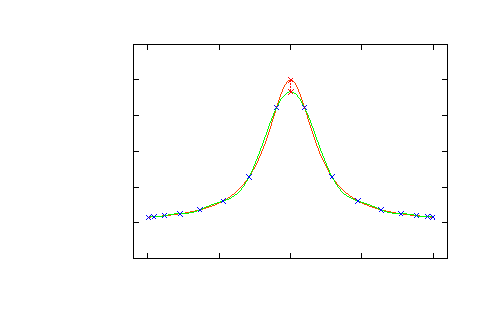
\includegraphics{16-cheb}}%
    \gplfronttext
  \end{picture}%
\endgroup

	% GNUPLOT: LaTeX picture with Postscript
\begingroup
  \makeatletter
  \providecommand\color[2][]{%
    \GenericError{(gnuplot) \space\space\space\@spaces}{%
      Package color not loaded in conjunction with
      terminal option `colourtext'%
    }{See the gnuplot documentation for explanation.%
    }{Either use 'blacktext' in gnuplot or load the package
      color.sty in LaTeX.}%
    \renewcommand\color[2][]{}%
  }%
  \providecommand\includegraphics[2][]{%
    \GenericError{(gnuplot) \space\space\space\@spaces}{%
      Package graphicx or graphics not loaded%
    }{See the gnuplot documentation for explanation.%
    }{The gnuplot epslatex terminal needs graphicx.sty or graphics.sty.}%
    \renewcommand\includegraphics[2][]{}%
  }%
  \providecommand\rotatebox[2]{#2}%
  \@ifundefined{ifGPcolor}{%
    \newif\ifGPcolor
    \GPcolortrue
  }{}%
  \@ifundefined{ifGPblacktext}{%
    \newif\ifGPblacktext
    \GPblacktextfalse
  }{}%
  % define a \g@addto@macro without @ in the name:
  \let\gplgaddtomacro\g@addto@macro
  % define empty templates for all commands taking text:
  \gdef\gplbacktext{}%
  \gdef\gplfronttext{}%
  \makeatother
  \ifGPblacktext
    % no textcolor at all
    \def\colorrgb#1{}%
    \def\colorgray#1{}%
  \else
    % gray or color?
    \ifGPcolor
      \def\colorrgb#1{\color[rgb]{#1}}%
      \def\colorgray#1{\color[gray]{#1}}%
      \expandafter\def\csname LTw\endcsname{\color{white}}%
      \expandafter\def\csname LTb\endcsname{\color{black}}%
      \expandafter\def\csname LTa\endcsname{\color{black}}%
      \expandafter\def\csname LT0\endcsname{\color[rgb]{1,0,0}}%
      \expandafter\def\csname LT1\endcsname{\color[rgb]{0,1,0}}%
      \expandafter\def\csname LT2\endcsname{\color[rgb]{0,0,1}}%
      \expandafter\def\csname LT3\endcsname{\color[rgb]{1,0,1}}%
      \expandafter\def\csname LT4\endcsname{\color[rgb]{0,1,1}}%
      \expandafter\def\csname LT5\endcsname{\color[rgb]{1,1,0}}%
      \expandafter\def\csname LT6\endcsname{\color[rgb]{0,0,0}}%
      \expandafter\def\csname LT7\endcsname{\color[rgb]{1,0.3,0}}%
      \expandafter\def\csname LT8\endcsname{\color[rgb]{0.5,0.5,0.5}}%
    \else
      % gray
      \def\colorrgb#1{\color{black}}%
      \def\colorgray#1{\color[gray]{#1}}%
      \expandafter\def\csname LTw\endcsname{\color{white}}%
      \expandafter\def\csname LTb\endcsname{\color{black}}%
      \expandafter\def\csname LTa\endcsname{\color{black}}%
      \expandafter\def\csname LT0\endcsname{\color{black}}%
      \expandafter\def\csname LT1\endcsname{\color{black}}%
      \expandafter\def\csname LT2\endcsname{\color{black}}%
      \expandafter\def\csname LT3\endcsname{\color{black}}%
      \expandafter\def\csname LT4\endcsname{\color{black}}%
      \expandafter\def\csname LT5\endcsname{\color{black}}%
      \expandafter\def\csname LT6\endcsname{\color{black}}%
      \expandafter\def\csname LT7\endcsname{\color{black}}%
      \expandafter\def\csname LT8\endcsname{\color{black}}%
    \fi
  \fi
    \setlength{\unitlength}{0.0500bp}%
    \ifx\gptboxheight\undefined%
      \newlength{\gptboxheight}%
      \newlength{\gptboxwidth}%
      \newsavebox{\gptboxtext}%
    \fi%
    \setlength{\fboxrule}{0.5pt}%
    \setlength{\fboxsep}{1pt}%
\begin{picture}(4534.00,2834.00)%
    \gplgaddtomacro\gplbacktext{%
      \csname LTb\endcsname%%
      \put(990,499){\makebox(0,0)[r]{\strut{}\num{-0.25}}}%
      \put(990,842){\makebox(0,0)[r]{\strut{}\num{0}}}%
      \put(990,1184){\makebox(0,0)[r]{\strut{}\num{0.25}}}%
      \put(990,1527){\makebox(0,0)[r]{\strut{}\num{0.5}}}%
      \put(990,1869){\makebox(0,0)[r]{\strut{}\num{0.75}}}%
      \put(990,2212){\makebox(0,0)[r]{\strut{}\num{1}}}%
      \put(990,2554){\makebox(0,0)[r]{\strut{}\num{1.25}}}%
      \put(1259,279){\makebox(0,0){\strut{}\num{-1}}}%
      \put(1944,279){\makebox(0,0){\strut{}\num{-0.5}}}%
      \put(2630,279){\makebox(0,0){\strut{}\num{0}}}%
      \put(3315,279){\makebox(0,0){\strut{}\num{0.5}}}%
      \put(4000,279){\makebox(0,0){\strut{}\num{1}}}%
      \put(2355,855){\makebox(0,0)[l]{\strut{}$ n = 32 $}}%
      \put(1670,1527){\makebox(0,0)[l]{\strut{}\color{red} \num{675}}}%
      \put(3315,1527){\makebox(0,0)[l]{\strut{}\color{red} \num{675}}}%
    }%
    \gplgaddtomacro\gplfronttext{%
    }%
    \gplbacktext
    \put(0,0){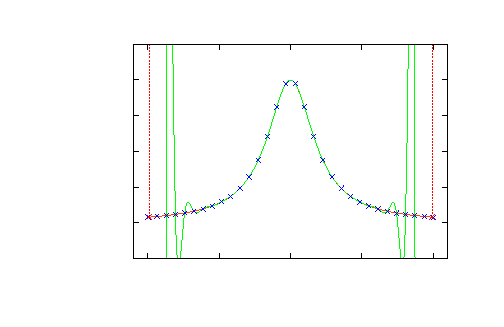
\includegraphics{32-eq}}%
    \gplfronttext
  \end{picture}%
\endgroup
% GNUPLOT: LaTeX picture with Postscript
\begingroup
  \makeatletter
  \providecommand\color[2][]{%
    \GenericError{(gnuplot) \space\space\space\@spaces}{%
      Package color not loaded in conjunction with
      terminal option `colourtext'%
    }{See the gnuplot documentation for explanation.%
    }{Either use 'blacktext' in gnuplot or load the package
      color.sty in LaTeX.}%
    \renewcommand\color[2][]{}%
  }%
  \providecommand\includegraphics[2][]{%
    \GenericError{(gnuplot) \space\space\space\@spaces}{%
      Package graphicx or graphics not loaded%
    }{See the gnuplot documentation for explanation.%
    }{The gnuplot epslatex terminal needs graphicx.sty or graphics.sty.}%
    \renewcommand\includegraphics[2][]{}%
  }%
  \providecommand\rotatebox[2]{#2}%
  \@ifundefined{ifGPcolor}{%
    \newif\ifGPcolor
    \GPcolortrue
  }{}%
  \@ifundefined{ifGPblacktext}{%
    \newif\ifGPblacktext
    \GPblacktextfalse
  }{}%
  % define a \g@addto@macro without @ in the name:
  \let\gplgaddtomacro\g@addto@macro
  % define empty templates for all commands taking text:
  \gdef\gplbacktext{}%
  \gdef\gplfronttext{}%
  \makeatother
  \ifGPblacktext
    % no textcolor at all
    \def\colorrgb#1{}%
    \def\colorgray#1{}%
  \else
    % gray or color?
    \ifGPcolor
      \def\colorrgb#1{\color[rgb]{#1}}%
      \def\colorgray#1{\color[gray]{#1}}%
      \expandafter\def\csname LTw\endcsname{\color{white}}%
      \expandafter\def\csname LTb\endcsname{\color{black}}%
      \expandafter\def\csname LTa\endcsname{\color{black}}%
      \expandafter\def\csname LT0\endcsname{\color[rgb]{1,0,0}}%
      \expandafter\def\csname LT1\endcsname{\color[rgb]{0,1,0}}%
      \expandafter\def\csname LT2\endcsname{\color[rgb]{0,0,1}}%
      \expandafter\def\csname LT3\endcsname{\color[rgb]{1,0,1}}%
      \expandafter\def\csname LT4\endcsname{\color[rgb]{0,1,1}}%
      \expandafter\def\csname LT5\endcsname{\color[rgb]{1,1,0}}%
      \expandafter\def\csname LT6\endcsname{\color[rgb]{0,0,0}}%
      \expandafter\def\csname LT7\endcsname{\color[rgb]{1,0.3,0}}%
      \expandafter\def\csname LT8\endcsname{\color[rgb]{0.5,0.5,0.5}}%
    \else
      % gray
      \def\colorrgb#1{\color{black}}%
      \def\colorgray#1{\color[gray]{#1}}%
      \expandafter\def\csname LTw\endcsname{\color{white}}%
      \expandafter\def\csname LTb\endcsname{\color{black}}%
      \expandafter\def\csname LTa\endcsname{\color{black}}%
      \expandafter\def\csname LT0\endcsname{\color{black}}%
      \expandafter\def\csname LT1\endcsname{\color{black}}%
      \expandafter\def\csname LT2\endcsname{\color{black}}%
      \expandafter\def\csname LT3\endcsname{\color{black}}%
      \expandafter\def\csname LT4\endcsname{\color{black}}%
      \expandafter\def\csname LT5\endcsname{\color{black}}%
      \expandafter\def\csname LT6\endcsname{\color{black}}%
      \expandafter\def\csname LT7\endcsname{\color{black}}%
      \expandafter\def\csname LT8\endcsname{\color{black}}%
    \fi
  \fi
    \setlength{\unitlength}{0.0500bp}%
    \ifx\gptboxheight\undefined%
      \newlength{\gptboxheight}%
      \newlength{\gptboxwidth}%
      \newsavebox{\gptboxtext}%
    \fi%
    \setlength{\fboxrule}{0.5pt}%
    \setlength{\fboxsep}{1pt}%
\begin{picture}(4534.00,2834.00)%
    \gplgaddtomacro\gplbacktext{%
      \csname LTb\endcsname%%
      \put(990,499){\makebox(0,0)[r]{\strut{}\num{-0.25}}}%
      \put(990,842){\makebox(0,0)[r]{\strut{}\num{0}}}%
      \put(990,1184){\makebox(0,0)[r]{\strut{}\num{0.25}}}%
      \put(990,1527){\makebox(0,0)[r]{\strut{}\num{0.5}}}%
      \put(990,1869){\makebox(0,0)[r]{\strut{}\num{0.75}}}%
      \put(990,2212){\makebox(0,0)[r]{\strut{}\num{1}}}%
      \put(990,2554){\makebox(0,0)[r]{\strut{}\num{1.25}}}%
      \put(1259,279){\makebox(0,0){\strut{}\num{-1}}}%
      \put(1944,279){\makebox(0,0){\strut{}\num{-0.5}}}%
      \put(2630,279){\makebox(0,0){\strut{}\num{0}}}%
      \put(3315,279){\makebox(0,0){\strut{}\num{0.5}}}%
      \put(4000,279){\makebox(0,0){\strut{}\num{1}}}%
      \put(2355,855){\makebox(0,0)[l]{\strut{}$ n = 32 $}}%
    }%
    \gplgaddtomacro\gplfronttext{%
    }%
    \gplbacktext
    \put(0,0){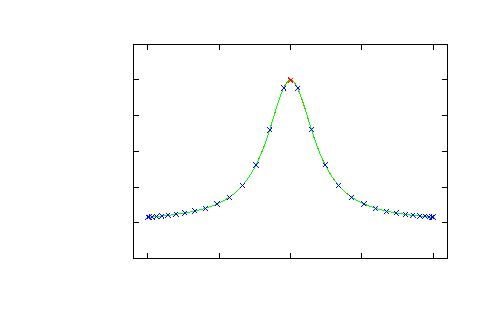
\includegraphics{32-cheb}}%
    \gplfronttext
  \end{picture}%
\endgroup

	\caption{Resultat d'interpolar \( f \) fent servir \( n \) nodes equidistants (esquerra) i \( n \) nodes de Chebyshev (dreta)}
	\label{fig:interpolacio}
\end{figure}
L'objectiu d'aquest problema és interpolar la funció \( f \colon \R \to \R \) donada per
\begin{equation*}
	f(x) = \frac{1}{1 + 25x^2}
\end{equation*}
a l'interval \( [-1,1] \) mitjançant el polinomi interpolador de Lagrange. Es faran servir dos conjunts de nodes diferents per a realitzar la interpolació. En primer lloc, \( n \) nodes equidistants dins de l'interval, és a dir, donats per
\begin{equation*}
	x_k = -1 + \frac{2k}{n}
\end{equation*}
per \( k \in \{0, \cdots, n-1\} \). Els altres nodes que farem servir seran nodes de Chebyshev, definits com
\begin{equation*}
	x_k = \cos{\left(\frac{2k+1}{n+1} \frac{\pi}{2}\right)}
\end{equation*}
per \( k \in \{0, \cdots, n-1\} \). Es proposa fer la interpolació fent servir 4, 8, 16, 32 i 64 nodes. 

El programa \texttt{nodes.c} genera una llista amb \( n \) nodes equidistants o de Chebyshev. Aquesta llista serveix d'entrada per al programa \texttt{prob1.c}, que implementa el mètode de diferències dividides de Newton per a calcular els coeficients del polinomi interpolador de Lagrange per als nodes donats. A més avalua aquest polinomi aplicant la regla de Horner. El fitxer auxiliar \texttt{diferencies\_dividides.c} conté la implementació de funcions auxiliars per aquests programes, com el càlcul de diferències dividides fent ús de l'expressió recursiva així com una implementació de la regla de Horner per avaluar un polinomi. 


\parbreak

Per a tenir una idea del màxim error que es comet en cada cas hem avaluat tant la funció com el polinomi en un nombre elevat de punts. En particular en els punts donats per \( x_k = \num{-0.989} + k \cdot \num{0.011} \) per \( k \in \{0, \cdots, 180\} \), que són 181 punts repartits de forma equidistant a l'interval on estem interpolant.  

\newpage

\section{Problema 2}
Considerem la funció de Bessel de primera espècie d'ordre zero, $J_0(x)$. Volem estimar els valors de les arrels de \( J_0 \), és a dir, de les \( x^{\ast} \) tals que \( J_0(x^{\ast}) = 0 \). Una manera de fer-ho és interpolar la inversa de \( J_0 \) a l'interval \( (1.9, 3) \). En aquest interval \( J_0 \) és localment invertible ja que és estrictament decreixent i derivable. Concretament construirem el polinomi interpolador que té per nodes \( (J_0(x_n), x_n) \). D'aquesta manera, si \( p \) és el polinomi que obtenim, \( p(0) \) és una aproximació de \( x^{\ast} \).

El programa \texttt{prob2.c} calcula el polinomi interpolador de Lagrange amb el mètode de les diferències dividides de Newton a partitr d'un conjunt de nodes donats. Seguidament l'avalua al punt zero fent servir la regla de Horner. La interpolació s'ha fet de grau 1, 3 i 5 i els resultats es mostren a 

\begin{table}[htb]
	\sffamily \small	\centering
	\caption{Interpolant valors positius de $J_0(x)$ més pròxims al canvi de signe de la funció.}	
	\begin{tabular}{cS[table-parse-only]S[table-parse-only]}
		\toprule
		{Grau} & { \( x^{\ast} \) } & { \( J_0(x^{\ast}) \) } \\
		\midrule
		1 & 2.404728613882804 & 5.03291522479392d-5\\
		3 & 2.404822718113948 & 1.47416266795862d-6\\
		5 & 2.404825294785460 & 1.36489238329446d-7\\
	\end{tabular}
\end{table}

\begin{table}[htb]
	\sffamily \small	\centering
	\caption{Interpolant valors negatius de $J_0(x)$ més pròxims al canvi de signe de la funció.}	
	\begin{tabular}{cS[table-parse-only]S[table-parse-only]}
		\toprule
		{Grau} & { \( x^{\ast} \) } & { \( J_0(x^{\ast}) \) } \\
		\midrule
		1 & 2.400077241947102 & 2.46750381340249d-3\\
		3 & 2.404149375353531 & 3.51087705194527d-4\\
		5 & 2.404216734868258 & 3.16108843546827d-4\\
	\end{tabular}
\end{table}

\begin{table}[htb]
	\sffamily \small	\centering
	\caption{Interpolant valors de $J_0(x)$ simètrics al canvi de signe de la funció.}	
	\begin{tabular}{cS[table-parse-only]S[table-parse-only]}
		\toprule
		{Grau} & { \( x^{\ast} \) } & { \( J_0(x^{\ast}) \) } \\
		\midrule
		1 & 2.404927513002775 & -5.29287203952310d-5\\
		3 & 2.404824021911155 & 7.97298995297100d-8\\
		5 & 2.404825653043717 & -4.94996456864148d-8\\
	\end{tabular}
\end{table}

Observem que el millor resultat l'obtenim amb la interpolació de grau 5 de valors simètrics al voltant del canvi de signe de $J_0(x)$. En general les millors són les interpolacions amb els valors positius i amb els simètrics, i la interpolació amb valors negatius és prou dolenta en comparació.

De fet ja podíem esperar des del principi que la millor interpolació fos la simètrica, ja que és l'única que en l'interval de punts interpoladors conté al $x^*$, i en general si tenim els punts interpoladors en un interval $[a,b]$ i volem avaluar el polinomi interpolador $p(x)$ en un punt fora d'aquest interval, l'error obtingut pot ser molt gran.

\newpage

\section{Problema 3}
El nostre objectiu és obtenir un valor aproximat de la integral
\begin{equation}\label{eq:integral}
	I=\int^{1}_0\dfrac{dx}{1+x^2} = \arctan(1) - \arctan(0) = \frac{1}{4}\pi \approx \num{0.785398163397448}
\end{equation}
pel mètode dels trapezis i pel mètode de Simpson dividint l'interval $[0,1]$ en quatre parts iguals.

El programa \texttt{prob3.c} calcula aquestes aproximacions i l'error que es comet amb cadascuna. Amb el mètode dels trapezis hem obtingut $I \approx \num{0.782794117647059}$, que comparat amb el valor exacte amb $15$ decimals de l'\cref{eq:integral} ens dóna un error aproximat de $\num{2.604045750389d-3}$.


Amb el mètode de Simpson obtenim $I \approx \num{0.785392156862745}$, que comparat amb l'\cref{eq:integral} té un error aproximat de $\num{6.006534703d-6}$.

Per tant veiem que amb la regla de Simpson hem obtingut una millor aproximació.

\newpage

\section{Problema 4}
El nostre objectiu és obtenir un valor aproximat de la integral
\begin{equation*}
	I=\int^{5}_1 \dfrac{e^x}{x} \,dx
\end{equation*}
pel mètode dels trapezis dividint l'interval $[1,5]$ en $n=4, 8, 16, 32, 64$ parts iguals.

El programa \texttt{prob4.c} calcula aquestes aproximacions i una estimació de l'error comés. Els resultats obtinguts per a cada $n$ es mostren a la \cref{tab:resultats}. 

\begin{table}[h]
	\centering \sffamily \small
	\caption{Resultat i estimació de l'error obtingut per a cada \( n \).}	
	\label{tab:resultats}
	\begin{tabular}{cS[table-parse-only]S[table-parse-only]}
		\toprule
		{ \( n \) } & {Aproximació de \( I \) } & { Estimació de l'error } \\
		\midrule
		4 & 40.239701356634455 & 10\\
		8 & 38.782928156314796 & 2.5\\
		16 & 38.413711363539406 & 0.625\\
		32 & 38.321069162332130 & 0.15625\\
		64 & 38.297886904128802 & 0.0390625\\
	\end{tabular}
\end{table}

L'estimació de l'error l'hem calculat segons la fórmula:
\begin{equation*}
	\abs{\dfrac{(b-a)F}{12}h^2},
\end{equation*}
on $b$ i $a$ són els extrems del interval ---en el nostre cas $b=5$ i $a=1$---, $F$ és una fita superior de la segona derivada de la funció que volem integrar a l'interval, i $h=(b-a)/n$. Tenim, per tot \( x \geq 1 \) 
\begin{equation*}
	\frac{d^2}{dx^2}\left(\frac{e^x}{x}\right) = \dfrac{e^x(x^3-2x^2+2x)}{x^4} \leq \dfrac{e^x}{x},
\end{equation*}
per tant podem triar $F=e^5/5 \approx 30$. De manera que per a cada $n$ ens queda l'estimació de l'error \( 160 \cdot n^{-2} \). Observem que per a un major nombre de divisions del interval esperem millorar l'aproximació de $I$.

\newpage
\section{Problema 5}
Volem calcular amb un error menor que $10^{-2}$ el valor de la integral
\begin{equation*}
	I = \int_{1}^{2}\log(x) \, dx
\end{equation*}
utilitzant la regla composta de Simpson.

Una fita de l'error amb aquest mètode ve donada per:
\begin{equation*}
	\varepsilon = \abs{\dfrac{(b-a)F}{180}h^4 } 
\end{equation*}
on $b$, $a$ són els extrems del interval, $F$ és una fita superior al interval del valor absolut de la quarta derivada de la funció que volem integrar, i $h=(b-a)/n$ on $n$ és el nombre de divisions del interval que utilitzem. En el nostre cas $a=1$, $b=2$, $|f^{(4)}(x)|=|-6/x^4|\leq6$ per a $x\in[1,2]$, de manera que volem
\begin{equation*}
	10^{-2} \geq \abs{\frac{6}{180} \dfrac{1}{n^4}}. 
\end{equation*}
Per tant necessitarem fer com a mínim $n=2$ divisions del interval $[1,2]$ per a obtenir la precisió demanada.

El programa \texttt{prob5.c} calcula aquesta integral amb diversos valors per a $n$, els resultats obtinguts són els següents:
\begin{table}[htb]
	\centering
	\caption{Resultats per a diversos $n$ parells}	
	\begin{tabular}{cS[table-parse-only]}
		\toprule
		{ \( n \) } & {Aproximació de \( I \) } \\
		\midrule
		2 & 0.385834602165434 \\
		4 & 0.386259562814567 \\
		6 & 0.386287163278802 \\
		8 & 0.386292043466313 \\
	\end{tabular}
\end{table}\\
Observem que amb $n=2$ iteracions ja hem obtingut dues xifres decimals correctes, per tant la nostra estimació de l'error ha sigut adequada.

\newpage

\section{Problema 6}
En aquest problema se'ns dóna una sèrie de valors de temps i velocitat, i se'ns demana calcular l'espai recorregut. Volem doncs aproximar la integral:
\begin{equation*}
	L=\int_{0}^{84}v(t)dt,
\end{equation*}
per a la qual tenim valors discrets de $v(t)$ en intervals de temps de \SI{6}{s}. Per tant estem dividint l'interval $[0,84]$ en $n=14$ parts iguals. Per a trobar $L$ utilitzarem la regla de Simpson composta, ja que en general dóna un millor resultat que la regla composta dels trapezis. 

El programa \texttt{prob6.c} calcula aquesta aproximació. El resultat que obtenim és \( L = \SI{2909.400000000000091}{m} \), per tant la pista mesura aproximadament \SI{2909}{km}.

\newpage
\section{Problema 7}
\begin{figure}[htb]
	\centering
	\sffamily \footnotesize
	% GNUPLOT: LaTeX picture with Postscript
\begingroup
  \makeatletter
  \providecommand\color[2][]{%
    \GenericError{(gnuplot) \space\space\space\@spaces}{%
      Package color not loaded in conjunction with
      terminal option `colourtext'%
    }{See the gnuplot documentation for explanation.%
    }{Either use 'blacktext' in gnuplot or load the package
      color.sty in LaTeX.}%
    \renewcommand\color[2][]{}%
  }%
  \providecommand\includegraphics[2][]{%
    \GenericError{(gnuplot) \space\space\space\@spaces}{%
      Package graphicx or graphics not loaded%
    }{See the gnuplot documentation for explanation.%
    }{The gnuplot epslatex terminal needs graphicx.sty or graphics.sty.}%
    \renewcommand\includegraphics[2][]{}%
  }%
  \providecommand\rotatebox[2]{#2}%
  \@ifundefined{ifGPcolor}{%
    \newif\ifGPcolor
    \GPcolortrue
  }{}%
  \@ifundefined{ifGPblacktext}{%
    \newif\ifGPblacktext
    \GPblacktextfalse
  }{}%
  % define a \g@addto@macro without @ in the name:
  \let\gplgaddtomacro\g@addto@macro
  % define empty templates for all commands taking text:
  \gdef\gplbacktext{}%
  \gdef\gplfronttext{}%
  \makeatother
  \ifGPblacktext
    % no textcolor at all
    \def\colorrgb#1{}%
    \def\colorgray#1{}%
  \else
    % gray or color?
    \ifGPcolor
      \def\colorrgb#1{\color[rgb]{#1}}%
      \def\colorgray#1{\color[gray]{#1}}%
      \expandafter\def\csname LTw\endcsname{\color{white}}%
      \expandafter\def\csname LTb\endcsname{\color{black}}%
      \expandafter\def\csname LTa\endcsname{\color{black}}%
      \expandafter\def\csname LT0\endcsname{\color[rgb]{1,0,0}}%
      \expandafter\def\csname LT1\endcsname{\color[rgb]{0,1,0}}%
      \expandafter\def\csname LT2\endcsname{\color[rgb]{0,0,1}}%
      \expandafter\def\csname LT3\endcsname{\color[rgb]{1,0,1}}%
      \expandafter\def\csname LT4\endcsname{\color[rgb]{0,1,1}}%
      \expandafter\def\csname LT5\endcsname{\color[rgb]{1,1,0}}%
      \expandafter\def\csname LT6\endcsname{\color[rgb]{0,0,0}}%
      \expandafter\def\csname LT7\endcsname{\color[rgb]{1,0.3,0}}%
      \expandafter\def\csname LT8\endcsname{\color[rgb]{0.5,0.5,0.5}}%
    \else
      % gray
      \def\colorrgb#1{\color{black}}%
      \def\colorgray#1{\color[gray]{#1}}%
      \expandafter\def\csname LTw\endcsname{\color{white}}%
      \expandafter\def\csname LTb\endcsname{\color{black}}%
      \expandafter\def\csname LTa\endcsname{\color{black}}%
      \expandafter\def\csname LT0\endcsname{\color{black}}%
      \expandafter\def\csname LT1\endcsname{\color{black}}%
      \expandafter\def\csname LT2\endcsname{\color{black}}%
      \expandafter\def\csname LT3\endcsname{\color{black}}%
      \expandafter\def\csname LT4\endcsname{\color{black}}%
      \expandafter\def\csname LT5\endcsname{\color{black}}%
      \expandafter\def\csname LT6\endcsname{\color{black}}%
      \expandafter\def\csname LT7\endcsname{\color{black}}%
      \expandafter\def\csname LT8\endcsname{\color{black}}%
    \fi
  \fi
    \setlength{\unitlength}{0.0500bp}%
    \ifx\gptboxheight\undefined%
      \newlength{\gptboxheight}%
      \newlength{\gptboxwidth}%
      \newsavebox{\gptboxtext}%
    \fi%
    \setlength{\fboxrule}{0.5pt}%
    \setlength{\fboxsep}{1pt}%
\begin{picture}(4534.00,2834.00)%
    \gplgaddtomacro\gplbacktext{%
      \csname LTb\endcsname%%
      \put(990,499){\makebox(0,0)[r]{\strut{}\num{-0.25}}}%
      \put(990,842){\makebox(0,0)[r]{\strut{}\num{0}}}%
      \put(990,1184){\makebox(0,0)[r]{\strut{}\num{0.25}}}%
      \put(990,1527){\makebox(0,0)[r]{\strut{}\num{0.5}}}%
      \put(990,1869){\makebox(0,0)[r]{\strut{}\num{0.75}}}%
      \put(990,2212){\makebox(0,0)[r]{\strut{}\num{1}}}%
      \put(990,2554){\makebox(0,0)[r]{\strut{}\num{1.25}}}%
      \put(1259,279){\makebox(0,0){\strut{}\num{-1}}}%
      \put(1944,279){\makebox(0,0){\strut{}\num{-0.5}}}%
      \put(2630,279){\makebox(0,0){\strut{}\num{0}}}%
      \put(3315,279){\makebox(0,0){\strut{}\num{0.5}}}%
      \put(4000,279){\makebox(0,0){\strut{}\num{1}}}%
      \put(2355,855){\makebox(0,0)[l]{\strut{}$ n = 4 $}}%
    }%
    \gplgaddtomacro\gplfronttext{%
    }%
    \gplbacktext
    \put(0,0){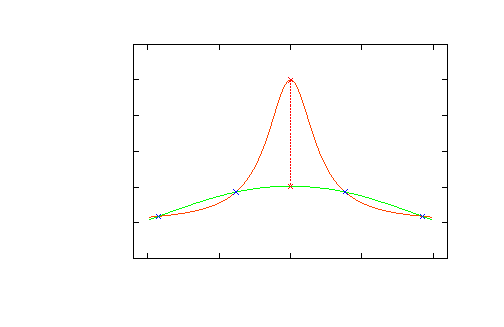
\includegraphics{04-splines}}%
    \gplfronttext
  \end{picture}%
\endgroup
% GNUPLOT: LaTeX picture with Postscript
\begingroup
  \makeatletter
  \providecommand\color[2][]{%
    \GenericError{(gnuplot) \space\space\space\@spaces}{%
      Package color not loaded in conjunction with
      terminal option `colourtext'%
    }{See the gnuplot documentation for explanation.%
    }{Either use 'blacktext' in gnuplot or load the package
      color.sty in LaTeX.}%
    \renewcommand\color[2][]{}%
  }%
  \providecommand\includegraphics[2][]{%
    \GenericError{(gnuplot) \space\space\space\@spaces}{%
      Package graphicx or graphics not loaded%
    }{See the gnuplot documentation for explanation.%
    }{The gnuplot epslatex terminal needs graphicx.sty or graphics.sty.}%
    \renewcommand\includegraphics[2][]{}%
  }%
  \providecommand\rotatebox[2]{#2}%
  \@ifundefined{ifGPcolor}{%
    \newif\ifGPcolor
    \GPcolortrue
  }{}%
  \@ifundefined{ifGPblacktext}{%
    \newif\ifGPblacktext
    \GPblacktextfalse
  }{}%
  % define a \g@addto@macro without @ in the name:
  \let\gplgaddtomacro\g@addto@macro
  % define empty templates for all commands taking text:
  \gdef\gplbacktext{}%
  \gdef\gplfronttext{}%
  \makeatother
  \ifGPblacktext
    % no textcolor at all
    \def\colorrgb#1{}%
    \def\colorgray#1{}%
  \else
    % gray or color?
    \ifGPcolor
      \def\colorrgb#1{\color[rgb]{#1}}%
      \def\colorgray#1{\color[gray]{#1}}%
      \expandafter\def\csname LTw\endcsname{\color{white}}%
      \expandafter\def\csname LTb\endcsname{\color{black}}%
      \expandafter\def\csname LTa\endcsname{\color{black}}%
      \expandafter\def\csname LT0\endcsname{\color[rgb]{1,0,0}}%
      \expandafter\def\csname LT1\endcsname{\color[rgb]{0,1,0}}%
      \expandafter\def\csname LT2\endcsname{\color[rgb]{0,0,1}}%
      \expandafter\def\csname LT3\endcsname{\color[rgb]{1,0,1}}%
      \expandafter\def\csname LT4\endcsname{\color[rgb]{0,1,1}}%
      \expandafter\def\csname LT5\endcsname{\color[rgb]{1,1,0}}%
      \expandafter\def\csname LT6\endcsname{\color[rgb]{0,0,0}}%
      \expandafter\def\csname LT7\endcsname{\color[rgb]{1,0.3,0}}%
      \expandafter\def\csname LT8\endcsname{\color[rgb]{0.5,0.5,0.5}}%
    \else
      % gray
      \def\colorrgb#1{\color{black}}%
      \def\colorgray#1{\color[gray]{#1}}%
      \expandafter\def\csname LTw\endcsname{\color{white}}%
      \expandafter\def\csname LTb\endcsname{\color{black}}%
      \expandafter\def\csname LTa\endcsname{\color{black}}%
      \expandafter\def\csname LT0\endcsname{\color{black}}%
      \expandafter\def\csname LT1\endcsname{\color{black}}%
      \expandafter\def\csname LT2\endcsname{\color{black}}%
      \expandafter\def\csname LT3\endcsname{\color{black}}%
      \expandafter\def\csname LT4\endcsname{\color{black}}%
      \expandafter\def\csname LT5\endcsname{\color{black}}%
      \expandafter\def\csname LT6\endcsname{\color{black}}%
      \expandafter\def\csname LT7\endcsname{\color{black}}%
      \expandafter\def\csname LT8\endcsname{\color{black}}%
    \fi
  \fi
    \setlength{\unitlength}{0.0500bp}%
    \ifx\gptboxheight\undefined%
      \newlength{\gptboxheight}%
      \newlength{\gptboxwidth}%
      \newsavebox{\gptboxtext}%
    \fi%
    \setlength{\fboxrule}{0.5pt}%
    \setlength{\fboxsep}{1pt}%
\begin{picture}(4534.00,2834.00)%
    \gplgaddtomacro\gplbacktext{%
      \csname LTb\endcsname%%
      \put(990,499){\makebox(0,0)[r]{\strut{}\num{-0.25}}}%
      \put(990,842){\makebox(0,0)[r]{\strut{}\num{0}}}%
      \put(990,1184){\makebox(0,0)[r]{\strut{}\num{0.25}}}%
      \put(990,1527){\makebox(0,0)[r]{\strut{}\num{0.5}}}%
      \put(990,1869){\makebox(0,0)[r]{\strut{}\num{0.75}}}%
      \put(990,2212){\makebox(0,0)[r]{\strut{}\num{1}}}%
      \put(990,2554){\makebox(0,0)[r]{\strut{}\num{1.25}}}%
      \put(1259,279){\makebox(0,0){\strut{}\num{-1}}}%
      \put(1944,279){\makebox(0,0){\strut{}\num{-0.5}}}%
      \put(2630,279){\makebox(0,0){\strut{}\num{0}}}%
      \put(3315,279){\makebox(0,0){\strut{}\num{0.5}}}%
      \put(4000,279){\makebox(0,0){\strut{}\num{1}}}%
      \put(2355,855){\makebox(0,0)[l]{\strut{}$ n = 4 $}}%
    }%
    \gplgaddtomacro\gplfronttext{%
    }%
    \gplbacktext
    \put(0,0){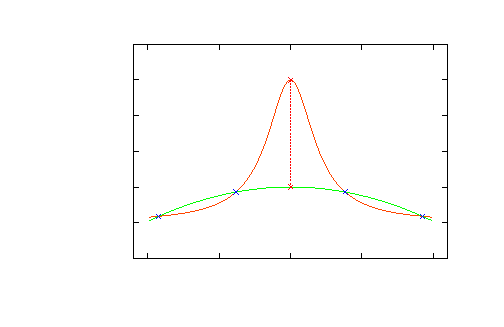
\includegraphics{04-cheb}}%
    \gplfronttext
  \end{picture}%
\endgroup

	\caption{Resultat d'interpolar \( f \) fent servir \( n \) nodes equidistants (esquerra) i \( n \) nodes de Chebyshev (dreta)}
	\label{fig:splines}	
\end{figure}

\end{document}
